%------------------------------------------------------------------------------
%	CAPITOLO 1
%------------------------------------------------------------------------------

\chapter{Amici Sinceri}
I reverendi don \index[Personaggi]{Don Salvatori Ruggero}Ruggero Salvatori\footnote{\textbf{Don Ruggero Salvatori} fu un rettore della Chiesa di Alfonsine. Era lo zio di \index[Personaggi]{Massaroli Giuseppe}Massaroli Giuseppe che sposò la marchesa \index[Personaggi]{Passari Santacroce Venturi Gallerani Giuditta (marchesa)}Giuditta Passari. Oltre ad essere presente nell'indice degli associati all'operetta "Memorie Storiche dell'Alfonsine" di Gian Francesco Rambelli, è noto il fatto che fosse presente al momento dell'assassinio del conte Camillo Foschini per opera di banditi.} e don \index[Personaggi]{Don Faggioli Paolo}Paolo Faggioli erano cresciuti insieme, fatti gli studi ed abbracciato la carriera ecclesiastica. La loro vocazione doveva dunque essere un atto di fede, amor del prossimo e carità cristiana.\\
\indent Bisognava però vivere ed ai piccoli proventi di stola bianca e nera aggiungere qualche altra cosa per il mantenimento decoroso delle famiglie, di relativi fratelli e nipoti, che sempre hanno spolpato i celibi... agiati. Anche in questo pensiero assillante furono d'accordo ed attuarono la speculazione di prendere insieme un podere in affitto di là da Po. Dove precisamente questa unione fraterna trovò le sue discrepanze fu nella divisione degli utili e dei prodotti del fondo\footnote{Il podere, la proprietà che avevano in comune}. \\
\indent Insieme da buoni amiconi, col tradizionale cavallo e biroccino\footnote{Biroccio: carretto porta persone trainato da un cavallo o un asino} si recarono un giorno sul fondo per dividere insieme al colono, il prodotto di un filare di meli. La sorpresa dei due indivisibili amiconi fu grande quando si trovarono a dividere un esiguo mucchietto di mele di scarto... invece della grande quantità conteggiata nella loro mente. \\
\indent Con motto istintivo e temporaneamente i due reverendi inveirono contro il povero colono, tacciandolo di ladro, disonesto... per aver rubato tutte le mele. Agli improperi ed onorifici titoli, seguivano poi le minacce d'escomio\footnote{Cessazione di locazione data a un colono o mezzadro e, anche, la sua esecuzione} da parte dei due reverendi inviperiti... con le faccie accese. Il colono minacciato buttò il dardo... contro le minaccie dei due amici per la pelle e rispose: \\
\indent <<Don \index[Personaggi]{Don Salvatori Ruggero}Ruggero mi ha ordinato di portargli a casa quattro sacchi di mele, senza che lo sappiate voi don \index[Personaggi]{Don Faggioli Paolo}Paolo. Voi don \index[Personaggi]{Don Faggioli Paolo}Paolo mi avete ordinato di portarvi quattro sacchi di mele. Senza che lo sappia don \index[Personaggi]{Don Salvatori Ruggero}Ruggero. Otto sacchi di mele vi ho portato, altri otto mi sono preso perché dovevano essere di mia parte... e questo è il resto delle mele... da dividere.>>\\
\indent I due reverendi amiconi man mano che il colono parlava e di credere che smettessero il cipiglio fiero e distendessero serenamente le rughe del volto\footnote{La frase è stata riportata fedelmente. Si intende che il colono fece capire ai due reverendi che era tutto uno scherzo, provocando una gran risata da parte dei due}... perché entrambi proruppero in una risata...aggiungendo: \\
\indent <<Credevo di farvela... invece mi avete prevenuto>>.
\begin{center}
\rule{1.5cm}{0.4pt}
\end{center}
Al tempo della vendemmia, ciascuno dei reverendi dispose per portarsi a casa un carro di buon'uva. Il mezzo della gabbatura fu mutato\footnote{Il modo in cui si fregarono a vicenda cambiò}. Due carra di buona uva ed altri due per il colono sul fondo non c'erano. Chi doveva aver la peggio è quel che vedremo. \\
\indent Nei discorsi in sacristia, don \index[Personaggi]{Don Salvatori Ruggero}Ruggero a don \index[Personaggi]{Don Faggioli Paolo}Paolo: 
<<Sentite un po' oggi l'uva è pronta per essere pigiata e portata a casa>>.\\
\indent Don \index[Personaggi]{Don Faggioli Paolo}Paolo: <<Io, non ci posso però andare, ci mando mio fratello per fare tutto.>>\\
\indent Don \index[Personaggi]{Don Salvatori Ruggero}Ruggero: <<Va bene, pensate pure voi; io sto a casa a far preparare il tino\footnote{Bacinella per pestare l'uva}>>.\\
\indent Verso sera don Ruggero era sugli spini, nell'attesa dell'uva andò sul \index[Luoghi]{Dall'Ara (palazzo)}Crocevia Dall'Ara\footnote{L'incrocio tra via \index[Luoghi]{Raspona (via)}Raspona e via \index[Luoghi]{Reale (via)}Reale su cui si affaccia il \textbf{Palazzo Dall'Ara} ancora oggi esistente, anche se in condizioni pessime. } ad aspettare i carri...che non si fecero molto aspettare. Appena apparvero i carri coi contadini don Ruggero li fermo e domandò: \\
\indent <<Tu dove devi andare?>>\\
\indent <<Da don Paolo>> rispose il contadino. \\
\indent <<E tu dall'altro carro, dove devi andare?>> \\
\indent <<Da voi, don Ruggero>>. \\
\indent Allora don \index[Personaggi]{Don Salvatori Ruggero}Ruggero, temendo uno scacco, col suo piano in testa tanto ruminato\footnote{Studiato, pensato}, ordinò ai coloni: \\
\indent <<Tu, invece di portare il tuo carro d'uva a don Paolo portala a me, e tu che devi venire da me, va da don Paolo>> ed ordinato ciò scortò il carro fino a casa sua.\\
\indent Le sorprese vennero alla svinatura del vino. Don \index[Personaggi]{Don Salvatori Ruggero}Ruggero va con la solita confidenza a casa di don \index[Personaggi]{Don Faggioli Paolo}Paolo e gli chiede: \\
\indent <<Fatemi sentire il vostro vino nuovo>>. \\
\indent Fu subito accontentato, anche perché lo sapevano un ghiottone impenitente.\\
\indent Così si svolse il seguito: don \index[Personaggi]{Don Salvatori Ruggero}Ruggero a don \index[Personaggi]{Don Faggioli Paolo}Paolo <<Ma com'è buono il vostro vino... mentre il mio è cattivo.>> \\
\indent Don Paolo scoppiò a ridere e rispose: <<Mio fratello ve l'ha fatta perché sapeva che non vi sareste fidato ed avreste disposto sempre il contrario. Ci siete caduto per colpa vostra!>>.\\
\indent Don \index[Personaggi]{Don Salvatori Ruggero}Ruggero (mortificato) rispose: <<Mi brucia, perché me l'ha fatta un imbecille.>>\\
\indent Aveva preso veramente cappello per lo scacco subito\footnote{Si era veramente offeso per il torto subito}, si piantò quindi il tricorno ecclesiastico in testa... e se ne andò a casa di umore più nero della sua veste.\\
\indent L'inganno avrebbe dovuto essergli stato teso da una mente pari alla sua per salvargli la reputazione di furbacchione.\\


 \begin{figure}[htb]
    \centering
    %\vspace{-0.7cm}
    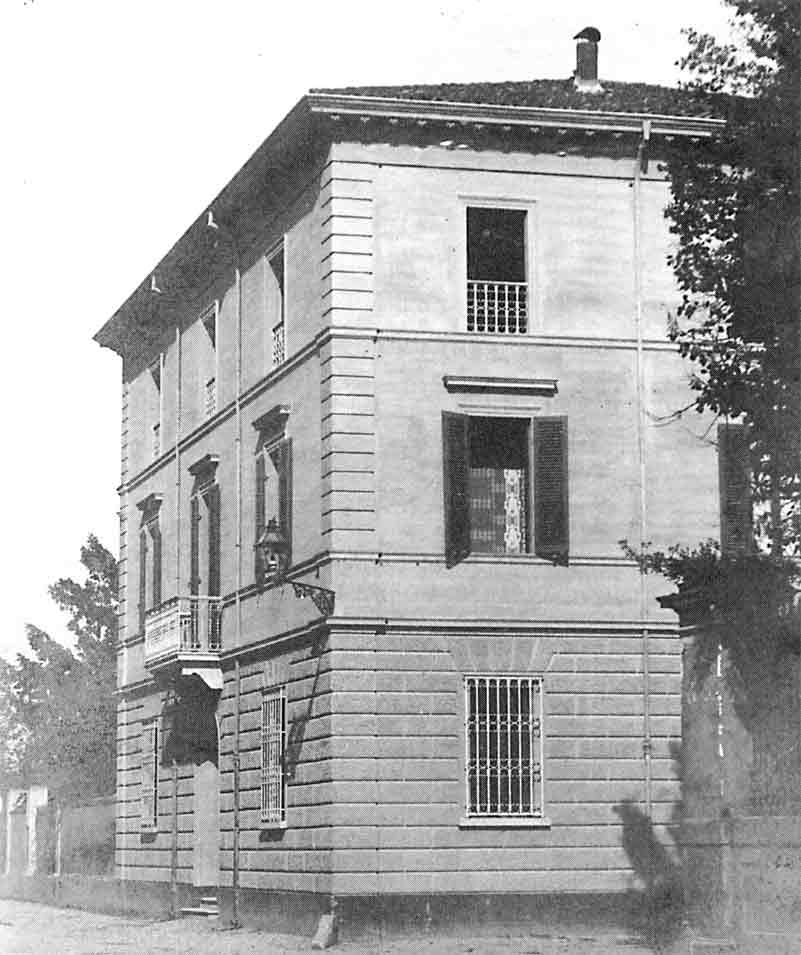
\includegraphics[width=\textwidth]{dallara}
    \caption*{Il palazzo appartenne a \index[Personaggi]{Dall'Ara Pietro}\textbf{Pietro Dall'Ara}, un medico dell'Università di Bologna, arrivato ad Alfonsine nel 1812 con una commissione di medici inviata appositamente per debellare un'epidemia malarica che aveva fatto ad Alfonsine già 300 vittime. Il Dottor Dall'Ara, originario di Reggio Emilia, riuscì a salvare molti alfonsinesi da quella perniciosa malattia, riuscendo a farsi benvolere, tanto che rimase ad Alfonsine e già nel 1832 fu nominato Priore (Sindaco) del Comune.\label{fig:dallara}}
    %\vspace{-0.3cm}
\end{figure}












































%